\subsection{Beyond accuracy: transparency, accountability, robustness and privacy}\label{sec:fat-exp}
\paragraph{Transparency: explanations and diagnosis (H5).}
Table~\ref{tab:fat} evaluates the class-level explanations against the ground truth. For label-swap groups the divergent classes reported by the server are \emph{exactly} the swapped classes in every pair of clusters (precision, recall and exact match $1.00$), and the diagnosis ``class-specific concept shift'' is always correct. A typical explanation reads: \emph{``cluster 0 vs.\ cluster 2: class-specific concept shift on classes [4, 5, 6, 7]''}, where group 2 swaps $4\leftrightarrow5$ and $6\leftrightarrow7$. For rotations, precision is again $1.00$: no class is reported as divergent when it is not. Recall is lower ($0.75$ for rotations, $0.78$ for \emph{Mixed + QS}). The misses are classes on which the two concepts are close at the reference model, such as nearly symmetric items under a $180^\circ$ rotation. Proposition~\ref{prop:expl} guarantees fidelity only for classes with enough pooled evidence and a separation $\Delta$, so these misses are within its scope, but they make the diagnosis ``global shift'' correct for only 43\% of the rotation pairs.

\begin{table}[!htbp]
\centering
\caption{Transparency and accountability (Fashion-MNIST, 3 seeds, default settings). Certificates: share of clients with a confident certificate, and share of correctly placed clients (no conflict with any member of their cluster) among confident and among uncertain certificates.}\label{tab:fat}
\small
\begin{tabular}{lccc}
\toprule
& Rotation & Label swap & Mixed + QS \\
\midrule
\multicolumn{4}{l}{\emph{Explanations: divergent classes between clusters}}\\
precision & 1.00 & 1.00 & 1.00 \\
recall & 0.75 & 1.00 & 0.78 \\
exact set / diagnosis correct & 0.43 & 1.00 & 0.33 \\
\midrule
\multicolumn{4}{l}{\emph{Certificates}}\\
share of confident certificates & 0.76 & 0.87 & 0.77 \\
correct among confident & 0.923 & 1.000 & 1.000 \\
correct among uncertain & 0.690 & 1.000 & 1.000 \\
\midrule
\multicolumn{4}{l}{\emph{Newcomers}}\\
known concept, correctly assigned & 0.96 & 0.96 & -- \\
novel concept, flagged as novel & 1.00 & 1.00 & -- \\
\bottomrule
\end{tabular}
\end{table}

\paragraph{Accountability: certificates, audit log, newcomers (H5).}
With the jackknife standard errors of Eq.~\eqref{eq:cert}, 76--87\% of the clients receive a confident certificate. Confident certificates are correct in all cases for label swaps and \emph{Mixed + QS}, and in 92.3\% of the cases for rotations, against 69.0\% for uncertain ones. Where every client is correctly placed, the uncertain certificates are therefore conservative, as the simulation of Section~\ref{sec:outputs} predicts; under rotations they do point to the clients whose placement is in doubt. A confident certificate is informative but not a guarantee, and we report it as an empirical rate, not as a coverage probability. In an exploratory analysis on the other small-CNN datasets (Table~\ref{tab:cert_ext} in Appendix~\ref{app:more}; 3 seeds), the same holds where the clustering works: on MNIST, KMNIST and EMNIST, 91--100\% of the confident certificates are correct. Where the reference model does not separate the groups, however, the certificates do not reveal the failure. On SVHN every client is placed in one cluster with a confident certificate, and every such certificate is wrong; on CIFAR-10 only 2--33\% of the confident certificates are correct. A certificate measures how well a client fits its cluster at the given reference model; it cannot detect that the reference model itself does not separate the concepts, which is the failure mode that the warm-up rule of Section~\ref{sec:warmup} addresses. Newcomers that join after clustering, using the frozen reference model, are assigned to the right cluster in 96\% of the cases, and clients with a concept never seen during clustering are reported as \emph{novel} in all cases.

\paragraph{Dependence on the reference model.} The reference model is trained on the clients that are then clustered. To test whether the partition depends on which clients trained it, we trained it on a random half of the clients, or on all clients except those of one concept group, and clustered all clients at that model (Table~\ref{tab:refmodel} in Appendix~\ref{app:more}; six Fashion-MNIST and MNIST scenarios, 3 seeds). We predicted that ARI would change by at most $0.05$ with a random half and that at most 5\% of the conflicting pairs involving an excluded group would be merged; both hold. With a random half, ARI changes by at most $0.05$ against the full reference model, and the label-only federation stays a single cluster; clients that did not train the model are placed slightly less well than those that did (ARI $0.91$--$1.00$ against $1.00$). A group that never contributed to the reference model is still separated: at most $1.1\%$ of the conflicting pairs that involve it are merged. In these scenarios the clustering does not hinge on which clients trained the reference model, as long as the model has learned the task; this does not extend to the datasets where it has not (Sections~\ref{sec:datasets} and~\ref{sec:warmup}).

\paragraph{Concept drift after clustering.} We tested the following drift procedure: after clustering, 10\% or 20\% of the clients switch to another concept group, the server recomputes all signatures at the same reference model, and every client whose similarity to its own cluster falls below $\tau$ is flagged (Table~\ref{tab:drift} in Appendix~\ref{app:more}). Every drifted client is detected (detection rate $1.00$ in all settings), but the predicted rate of at most 5\% false alarms is \emph{not} met: 31--67\% of the unchanged clients are also flagged, and 38--75\% of the drifted clients are reassigned to the cluster of their new group. The cause is that the drifted clients remain members of their old cluster and pull the bottleneck similarity of their former cluster-mates below $\tau$. In an exploratory analysis, computing each client's similarity only to the members that did not drift (in practice, members that kept a confident certificate) reduces the false-alarm rate to 1--4\% with detection unchanged. Drift detection therefore works, but needs an iterative rule that first removes the clients that changed.



\paragraph{Malicious clients.} DisCo-CFL has no defence against adversarial clients, and we measured what happens when $m\in\{1,2,4\}$ of 40 clients send manipulated signatures (Table~\ref{tab:byz} in Appendix~\ref{app:more}; no hypothesis was made). Random vectors have no split-half reliability and are flagged as low-evidence or anomalous in every run; sign-flipped signatures are isolated, alone or among themselves. Neither attack harms the clustering of the honest clients (ARI $0.95$--$0.96$, at most 0.4\% conflicting merges, as without attack). A client that copies the signature of an honest client from another group, however, is always merged into that group, without being flagged: the signature carries no information that could reveal the copy. Defending against such mimicry would need authentication of the signature or secure aggregation of the clustering step, which we leave open; Byzantine-robust aggregation~\citep{dang2026fortress} protects the training of the cluster models, not the clustering signal.



\paragraph{Privacy.}
Figure~\ref{fig:dp} shows the ARI of the clustering when the signatures are released with the Gaussian mechanism of Proposition~\ref{prop:dp} ($C_{\rm clip}=0.5$, $\delta=10^{-5}$). These results measure the utility cost of noising the clustering signal only; the warm-up and the cluster training are not private (Remark~\ref{rem:dp}). As Proposition~\ref{prop:dp}(iii) predicts, the \emph{raw} cosine collapses to ARI $\approx0$ at every noise level, with 22--40 clusters: the noise attenuates all similarities. With disattenuation the clustering degrades gradually, and more data per client buys more privacy, as the $h\propto\sigma_{\rm dp}$ term predicts. Recovery is only partial, however. With 1{,}500 samples per client, ARI is $0.75$ and $0.76$ (rotation and label swap) at $\varepsilon=10$, $0.58$ and $0.65$ at $\varepsilon=4.4$, and $0.41$ and $0.55$ at $\varepsilon=2$; with 400 samples it is at most $0.43$ at any noise level we tried. Strong privacy for the clustering signal therefore needs much larger clients than our benchmarks have.

\begin{figure}[!htbp]
\centering
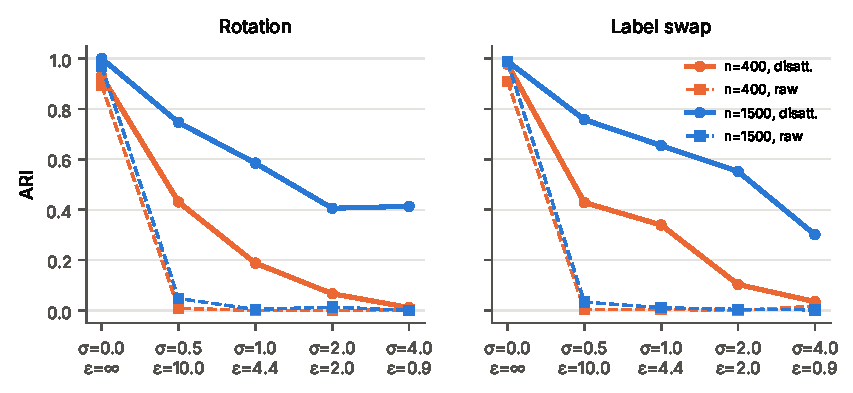
\includegraphics[width=0.85\linewidth]{dp.pdf}
\caption{Clustering quality under $(\varepsilon,10^{-5})$-DP signatures (3 seeds). Solid: DisCo-CFL; dashed: raw cosine. Orange: 400 samples per client; blue: 1{,}500.}\label{fig:dp}
\end{figure}

\paragraph{Class support.} The signatures reveal which classes a client holds (Section~\ref{sec:method}). Table~\ref{tab:support} (Appendix~\ref{app:more}) evaluates padding: under DP noise, every client also sends, for each class it does not hold, two independent noise vectors with the noise scale of its median class. Without padding the server knows the support exactly from the list of reported classes; even from the reliabilities alone ($R_i^c>0$) it would infer it with 77--92\% accuracy. With padding the list no longer reveals the support, but the reliabilities still do, with 63--84\% accuracy: a noise vector has a positive split-half correlation by chance in about 37\% of the cases, whereas a held class with enough data has a clearly positive one. Padding also costs clustering quality (ARI falls by up to $0.3$), because the noise classes add spurious evidence. It is therefore a weak mitigation. Hiding the support would need a mechanism that releases the support itself under DP, which we leave open.



\subsection{Calibration, sensitivity, ablation and cost}\label{sec:sens-cost}
\paragraph{Calibration and threshold (H3).}\label{sec:sens} Figure~\ref{fig:tau} varies $\tau$ on the clustering step. With disattenuation, ARI is $0.85$--$1.00$ for $\tau\in[0.85,0.95]$ in every concept-shift scenario, and the label-only scenario keeps $K=1$ up to $\tau=0.9$. With the raw cosine the useful range is narrower and higher thresholds over-split: at $\tau=0.95$ the label-only federation is split into 3 clusters and \emph{Rotation + QS} into 9.7 on average. Disattenuation therefore makes the threshold less sensitive towards high values, as H3 states. Towards low values the picture is reversed: at $\tau=0.8$ the raw cosine merges fewer groups than the disattenuated similarity (ARI $0.70$ against $0.60$ on \emph{Rotation}), because disattenuation raises all similarities, including those between groups. A calibrated scale thus shifts the useful range of $\tau$ upwards rather than widening it on both sides. The gain at the default threshold is moderate: without disattenuation (Table~\ref{tab:abl}) ARI drops by $0.04$--$0.11$ in the concept-shift scenarios and by $0.33$ in the label-only one. The sample-size study (Figure~\ref{fig:size} in Appendix~\ref{app:figs}) shows why. With clipped per-sample gradients, the raw cosine between clients of the same group is already $0.98$ on Fashion-MNIST, so there is little attenuation to correct; the disattenuated similarity is $0.99$--$1.00$. Attenuation becomes large under DP noise, where the raw cosine fails completely (Figure~\ref{fig:dp}). With very small clients (50--100 samples) both versions fail, for another reason: the groups become close at the reference model (between-group similarity $0.89$--$0.93$), i.e.\ the separation shrinks, and disattenuation does not help (ARI $0.13$--$0.63$, against $0.21$--$0.60$ for the raw cosine). Otsu's label-free threshold (Table~\ref{tab:diag}) lies at $0.76$--$0.83$ in the concept-shift scenarios. It recovers label swaps as well as $\tau=0.9$ (ARI $0.97$) but merges groups under rotations (ARI $0.58$--$0.71$). Over all scenarios (Table~\ref{tab:diag}) the comparison is two-sided. In the seven scenarios where DisCo-CFL fails (ARI below $0.5$), Otsu's threshold is better in four (e.g.\ Office-Home, $0.70$ against $0.26$; CIFAR-10 rotations with the pretrained network, $0.50$ against $0.07$), equal in the two SVHN scenarios and worse in one. In the 24 scenarios where DisCo-CFL succeeds it is lower in 19, equal in four and higher in one, and it splits single-concept federations (ARI $0$ in the label-only scenario). Its separation index $\eta$ does not distinguish successes from failures ($0.63$ for the $45^\circ$ rotation with ARI $1.00$, $0.73$ for CIFAR-10 label swaps with ARI $0.28$), so neither threshold dominates, and Otsu's rule does not replace $\tau$. The shrinkage $\lambda$ has almost no effect between $0.02$ and $1$ (Table~\ref{tab:lambda} in Appendix~\ref{app:figs}), including the values $0.02$ and $0.1$ that satisfy the condition of Corollary~\ref{cor:sc}.

\begin{figure}[!htbp]
\centering
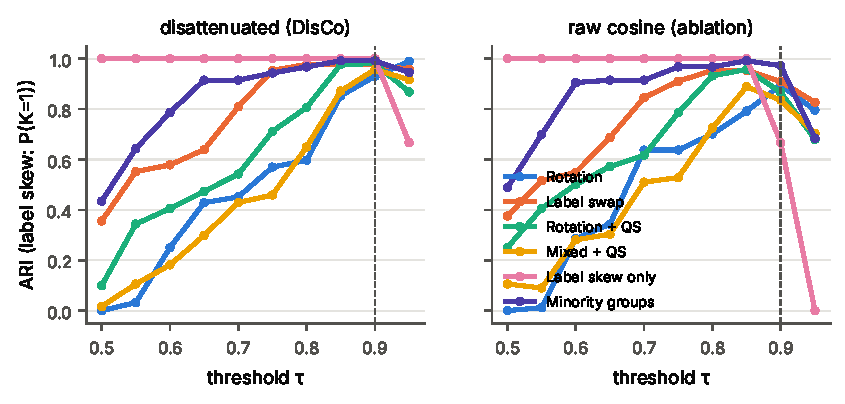
\includegraphics[width=0.85\linewidth]{tau_sensitivity.pdf}
\caption{Sensitivity to the threshold $\tau$ (3 seeds). The dashed line marks the default $\tau=0.9$, selected on the pilot runs (Section~\ref{sec:setup}).}\label{fig:tau}
\end{figure}

\paragraph{Edge cases.} The edge-case rules of Section~\ref{sec:method} were evaluated in three federations (Table~\ref{tab:edge} in Appendix~\ref{app:more}): the default minimum class size $m=4$ is best or close to best, the reliability floor $r_{\min}$ has no measurable effect, and extreme label skew ($\alpha=0.1$) or small clients lower ARI to about $0.7$.

\paragraph{Ablation (H3, H4).}
Table~\ref{tab:abl} removes one component at a time. Without class conditioning (one signature per client over all its data), clients are grouped by their label mix, the failure mode reported in the survey~\citep{benali2026survey}: 18--33 clusters and a concept accuracy 19 points lower. The mean linkage averages class-specific shifts away and merges conflicting clients (11.3\% on average, ARI $0.48$ under rotations), which supports H4: the minimum over classes matters. Linkage-ordered merging over-splits label swaps and \emph{Mixed + QS}. Without disattenuation or without clipping the federation is split more often, most visibly in the label-only scenario. Without the attachment stage, a noisy client stays alone in the label-only scenario in one of the three seeds. The table uses seeds 0--2 for all rows, so the DisCo-CFL row differs slightly from the five-seed means of Table~\ref{tab:main}. The ablation supports class conditioning and the bottleneck linkage clearly; evidence-ordered merging and clipping matter only in some scenarios (linkage-ordered merging is slightly better on \emph{Rotation}), and these two choices rest mainly on the pilot runs.

\begin{tableorg}[!htbp]
\centering
\caption{Ablation (Fashion-MNIST, 3 seeds): ARI / number of clusters $K$ per scenario, mean conflict-merge rate (\%) and mean concept accuracy (\%) over the five scenarios.}\label{tab:abl}
\scriptsize
\setlength{\tabcolsep}{3pt}
\resizebox{\textwidth}{!}{%
\begin{tabular}{lccccccc}
\toprule
Variant & Rotation & Label swap & Rot.\,+\,QS & Mixed\,+\,QS & Label only & Conflict\% & Concept \\
\midrule
DisCo-CFL (full) & 0.93 / 4.3 & 0.98 / 4.0 & 0.98 / 4.3 & 0.96 / 4.0 & 1.00 / 1.0 & 0.2 & 76.9 \\
without disattenuation (raw cosine) & 0.89 / 5.0 & 0.91 / 4.7 & 0.87 / 5.3 & 0.86 / 5.0 & 0.67 / 1.3 & 0.4 & 76.0 \\
without class conditioning & 0.05 / 31.7 & 0.04 / 32.7 & 0.03 / 33.0 & 0.02 / 29.0 & 0.00 / 17.7 & 0.8 & 57.9 \\
mean instead of bottleneck linkage & 0.48 / 3.0 & 0.70 / 4.0 & 0.79 / 4.0 & 0.58 / 4.0 & 1.00 / 1.0 & 11.3 & 73.6 \\
linkage-ordered merging & 0.95 / 4.7 & 0.85 / 5.3 & 0.97 / 4.3 & 0.77 / 6.3 & 0.67 / 1.3 & 0.0 & 75.7 \\
without per-sample clipping & 0.93 / 4.3 & 1.00 / 4.0 & 0.93 / 5.0 & 0.93 / 4.3 & 0.33 / 1.7 & 0.2 & 76.6 \\
without attachment stage & 0.91 / 5.0 & 0.98 / 4.0 & 0.97 / 4.7 & 0.96 / 4.0 & 0.67 / 1.3 & 0.1 & 76.7 \\
\bottomrule
\end{tabular}}
\end{tableorg}

\paragraph{Cost and scalability.}\label{sec:cost}
Table~\ref{tab:cost} reports wall-clock time per run and the floats each client uploads for clustering. Each DisCo-CFL client uploads its signature \emph{once}, $2p|S_i|\le2pC\approx2.0\times10^4$ floats with $p=1024$ ($1.8$--$2.0\times10^4$ on average for the default configuration in Table~\ref{tab:cost}), independent of the model dimension $d$ (46{,}730 for the small CNN, 8.4M for the ResNet-18 block). FL+HC and StoCFL upload $d$-dimensional updates or gradients for clustering, IFCA downloads $K$ models per client in every round, and FedCCFA exchanges classifiers and class anchors in every round. A DisCo-CFL run takes about as long as a FedAvg run (the times come from shared machines, so differences below about 20\% are noise; FedAvg-FT appears faster than FedAvg on the realistic benchmarks for this reason); StoCFL takes about twice as long because it trains two models per round. Computing the signature takes about 0.09\,s per client on one CPU core, and server-side clustering 0.09\,s for 40 clients and 6\,s for 320 clients. In the clustering-only scalability study, which uses 200 samples per client, ARI is $0.59$--$0.82$ for 40 to 320 clients. With 200 clients in the full pipeline (Table~\ref{tab:sweeps}) ARI is $0.88$ and accuracy is within $0.7$ points of the Oracle. The scalability study uses one seed per size and its ARI is not monotone in the number of clients, so it measures time rather than recovery.

\begin{tableorg}[!htbp]
\centering
\caption{Cost per run: mean wall-clock time (minutes; one CPU core for the small CNN, one GPU for the realistic benchmarks) and floats uploaded per client for the clustering signal. DisCo-AS: label-free warm-up (Section~\ref{sec:warmup}); DisCo-full: signature from the gradient of the whole layer-4 block (realistic benchmarks); DisCo-linkorder, DisCo-mean, DisCo-noClass, DisCo-noClip and DisCo-noDisatt: the ablation variants of Table~\ref{tab:abl} (linkage-ordered merging, mean linkage, without class conditioning, without clipping, without disattenuation).}\label{tab:cost}
{\scriptsize
\resizebox{\textwidth}{!}{%
\begin{tabular}{l c c c}
\toprule
Method & Time, small-CNN main (min) & Time, realistic (min) & Upload floats / client \\
\midrule
DisCo & 6.9 & 0.8 & 1.9e4 \\
DisCo-noAttach & 6.9 & 0.8 & 2.0e4 \\
DisCo-T30 & -- & 1.2 & 1.9e4 \\
FedAvg & 7.1 & 1.4 & 0 \\
Local & 6.9 & 1.4 & 0 \\
FedAvg-FT & 7.6 & 0.7 & 0 \\
IFCA & 11.0 & 2.6 & 0 \\
FeSEM & 7.7 & 1.5 & 0 \\
MTCFL & 6.1 & 0.8 & 0 \\
FL+HC & 7.6 & 1.6 & 2.0e6 \\
PACFL & 7.5 & 1.5 & 3.3e3 \\
StoCFL & 13.9 & 3.1 & 2.0e6 \\
StoCFL-W & 12.5 & 1.7 & 2.0e6 \\
FedCCFA & 5.2 & 5.8 & 5.9e5 \\
FedDAG-C & 7.9 & 1.5 & 5.8e4 \\
Oracle & 7.2 & 1.4 & 0 \\
DisCo-AS & 7.2 & -- & 1.5e4 \\
DisCo-full & -- & 1.8 & 3.7e4 \\
DisCo-linkorder & 6.3 & 1.1 & 1.8e4 \\
DisCo-mean & 6.0 & 1.2 & 1.8e4 \\
DisCo-noClass & 6.0 & 1.1 & 2.0e3 \\
DisCo-noClip & 5.9 & 1.2 & 1.8e4 \\
DisCo-noDisatt & 6.0 & 1.1 & 1.8e4 \\
\bottomrule
\end{tabular}}
}

\end{tableorg}
